\setchapterpreamble[u]{\margintoc}
\chapter{Conclusions}
\labch{conclusions}
\label{sec:conclusions}

In this dissertation, several methodologies have been presented for fusing information collected by multiple imaging sensors. The Enhanced Correlation Coefficient (\acrshort{ecc}) proposed by Evangelidis and Psarakis \cite{evangelidis_parametric_2008} is the baseline image-matching algorithm that helped to compose a multi-layer system. It had not been yet explored for the alignment of heterogeneous datasets in Remote Sensing, albeit suiting particularly well datasets with notable radiometric differences. It was demonstrated that the collected images depicting visible, infrared and multispectral wavelengths were accurately fused with an improved correlation coefficient. From here, this multi-layer system was translated to 3D point clouds to provide an easier-to-inspect representation for human operators. The most frequent estimation of 3D point clouds is to apply photogrammetric pipelines in open-source and commercial software. However, photogrammetry may lead to sparse point clouds with geometrical inaccuracies whether some kinds of imagery are used, for instance, thermal and multispectral datasets with low resolution. These drawbacks were tackled by estimating first a baseline point cloud from high-resolution \acrshort{rgb} imagery, using \acrshort{sfm}. Then, the rest of the matched information was projected into a dense \acrshort{rgb} point cloud, thereby achieving a multi-layer system in 3D. Albeit not being addressed before, hyperspectral swaths were also projected to this multi-layer model. However, it required a different pipeline due to the particularities of the viewing mechanism in push broom sensors. Therefore, the results were 2.5D heightfields rather than 3D point clouds. 

It was explained that other kinds of sensors, such as \acrshort{lidar} were way more prohibitive than the previously used imaging devices. Furthermore, attaching data to the observed data and generated products, such as semantic annotations, is a tedious task that involves time-consuming stages, including cleaning, manual annotations, etc. An alternative is to partially or entirely replace datasets acquired by real sensors with others generated in a computer. It requires emulating how real sensors behave to generate synthetic datasets which can be augmented with any kind of information. Emulating imaging sensors is feasible, mainly with the rising importance of Generative Adversarial Networks, though the scope was narrowed to \acrshort{lidar} simulations. \acrshort{lidar} sensors were parameterized to cover a wide range of commercial devices and subsequently applied to generating large \acrshort{lidar} datasets. As a result, large airborne and terrestrial surveys were solved in a few minutes at most. The simulated point clouds were also improved by estimating radiometric information; a comparison of two different techniques on the computation of intensity were checked. From the results, both approaches were able to produce point clouds with very notable differences among distinct surfaces. 

Finally, the remotely sensed and generated products, either 2D or 3D, were utilized for several applications. First, \acrshort{lidar} simulations were used for the planning of scanning in buildings with improved objective functions that served as the core of several metaheuristics. Then, thermal maps and point clouds were applied to the identification of buried remains in an archaeological site. Finally, hyperspectral swaths were processed and split into patches for the classification of grapevine varieties using Deep Learning.

On a technical level, these last three years have considerably contributed to improving as a researcher. The work carried out has led to important results that have been published in top journals and conferences from the Remote Sensing field, while others are still under review. In addition, I have had the pleasure of contributing to other colleagues' work, and despite those publications not fitting in this dissertation, they have greatly contributed to broadening my knowledge of Computer Graphics in other fields which are not my main area of expertise. 

\section{Summary of contributions}

In the first part of this dissertation, a methodology for correcting and fusing images from multiple data sources at the image level was described. The Enhanced Correlation Coefficient was proposed as it was highly suitable for remotely sensed images sensible to different wavelength intervals. It behaved surprisingly well over datasets with significant radiometric differences. This method was massively applied to match visible, multispectral and infrared datasets. Furthermore, this image-matching algorithm was checked to highlight how efficient is it, since it provided remarkable results even for lower image dimensions and distortions, such as noise. In fact, partly missing some of the details helped in reducing significantly the response time. 

The image-matching procedure represents the baseline work of this dissertation. The advantages and disadvantages of working with images and point clouds have been highlighted throughout this dissertation. Accordingly, the latter is better for some specific applications as they enable visualizing one area at a glance, whereas location awareness is considerably improved for tasks performed by human operators. However, point clouds are not as helpful whether they are sparse or present geometrical inaccuracies. Therefore, a formal framework was presented for the generation of point clouds comprising visible, thermal and multispectral point clouds. A dense and large \acrshort{rgb} point cloud was first achieved using photogrammetry, whereas the rest of the datasets were projected into the former point cloud. It tackled most of the drawbacks of applying photogrammetry to thermal and multispectral imagery. Additionally, this pipeline was shown to outperform commercial software in terms of 1) response time, 2) density and 3) size. Projection, on the other hand, was aware of occlusion to achieve colourimetrically accurate results. This was handled using two methods; firstly, occlusion was handled with a traditional depth buffer, whereas the aggregation of remaining image samples in every 3D point was achieved using aggregation and penalty functions. The latter helped to compute aggregated colours that minimized the dissimilarity of such aggregation and the starting collection of samples. 

Besides projection and occlusion-aware considerations, this pipeline was implemented in the \acrshort{gpu} a similar fashion to commercial software, e.g., Agisoft Metashape and Pix4Dmapper. Yet, the proposed methodology outperformed these commercial solutions in terms of response time. Other enhancements were tested, such as the reordering of the point cloud either globally or in small groups, as suggested by Schutz et al. \cite{schutz_rendering_2021}. The tests carried out showed that globally reordering the point cloud significantly improved the response time, despite including the latency derived from sorting. On the other hand, shuffling the sorted point clouds using small groups did not achieve better results as the sorting plus shuffling overhead worsened the results of a single-launch process. 

The second part of this dissertation comprised the generation of hyperspectral point clouds, which to the best of our knowledge, had not been achieved previously, at least in outdoor scenarios. It required stitching the hyperspectral swaths and an \acrshort{rgb} orthomosaic to compose a hyperspectral orthomosaic. This was later projected onto the voxelization of a 3D point cloud, also coined as heightfields. This led to generating 2.5D products rather than 3D since hyperspectral datasets were collected with \textit{nadir} view direction. The \acrshort{gsd} was adapted to the resolution of hyperspectral imagery, and despite occlusion not being a drawback here, samples from overlapping swaths were aggregated into the heightfields according to aggregation and penalty functions. Given the large size of the resulting hypercube, it was compressed in the radiometric dimension by following the approach of Graciano et al. \cite{graciano_real-time_2018}. The majority of steps were implemented in the \acrshort{gpu}, and besides that, the aftermath of compressing the spectral heightfields was a data structure that was slightly harder to traverse in real time. Hence, this drawback was alleviated by composing images in multiple frames. Similar to previous work, the point cloud visualization was enhanced using \acrshort{opengl}'s compute shaders while taking advantage of modern extensions.

After fusing real-world information, the \acrshort{lidar} technology was simulated with the Time of Flight principle plus systematic and random errors described in the literature. Atmospheric particles, highly reflective surfaces or slope- and height-derived errors were emulated, whereas the synthetic sensor was parameterized so that it could be fed with the specifications of nowadays commercial sensors. Furthermore, previous work had already solved part of this and proposed to emulate \acrshort{lidar} to generate large datasets for Deep Learning. However, another key factor is the synthetic scenarios which are later scanned; in this work, these were procedurally generated to compute a large number of point clouds. The scenarios are first labelled and linked to materials according to name patterns which facilitates this manual task. For procedural scenes, this task is only performed once to build environments with varying distributions that follow some pre-defined rules. Nonetheless, static scenes were also included and can be labelled as explained. Finally, a comparison was established on the calculation of return intensity; first, it was modelled using traditional Computer Graphics \acrshort{brdf}s, and then, these were simulated using real-world measurements as obtained from a goniophotometer. The comparison with real-world point clouds is hard to establish, and therefore, the experiments were carried out by showing the histograms of scenarios with different materials. This simulation was entirely wrapped in the \acrshort{gpu} to supply rapid aerial and terrestrial surveys, from the generation of \acrshort{lidar} beams to scanning. 

Unlike previous \acrshort{lidar} simulators, the proposed one was intended to simulate terrestrial and airborne surveys. The first is the most common, whereas the latter has been barely addressed. Both are articulated over the interpolation of temporal locations from a path, either user-defined or automatically computed. However, airborne surveys also required the simulation of different scanning patterns, from which parallel, zigzag and elliptical patterns stand out. Simulations with multiple returns were also addressed as they are especially relevant to filter out canopy and vegetation in airborne missions. Similarly, bathymetric \acrshort{lidar}s were also included to scan shallow underwater areas. 

Datasets and results from previous chapters were utilized in practical case studies. Firstly, hyperspectral swaths were corrected and applied to the classification of seventeen grapevine varieties, either belonging to red or white variants. Traditional techniques, based on the correlation of spectral signatures, did not fit well on the classification of very similar spectral signatures. Instead, a Deep Learning network was explored for the classification of grapevine varieties, using state-of-the-art layers, such as Inception or spatial attention. Hypercubes were split into patches, whose size was tuned during experimentation, and they were reduced to a single label; hence, the classification of every sample was influenced by its neighbourhood. Not only this network was proven to perform well over \acrshort{uas} datasets, but it also was able to obtain results close to the the-start-of-the-art overall accuracy in satellite imagery. Then, thermal maps and point clouds were applied to inspect an archaeological site, where two anomalous areas were spotted in areas that may correspond to the location of buried towers. 

\section{Future work}

Remote sensing and Deep Learning fields are rapidly evolving, and yet, there exist some future investigations that should be explored from this work:
\begin{itemize}
    \item Image matching was performed using commodity hardware, and therefore, it was explored whether downscaling and blur led to better response time. Indeed, it offered similar results with lower latency. From here, it could be explored if a pyramid scheme, from lower to higher size, helps to obtain better results while yet obtaining a low latency. This way, larger transformations are computed from low-resolution imagery, whereas the most fine-grained changes are calculated with the starting dimensions. Besides reducing the response time, this approach could also help to match images with more notable differences.
    \begin{figure}
        \centering
        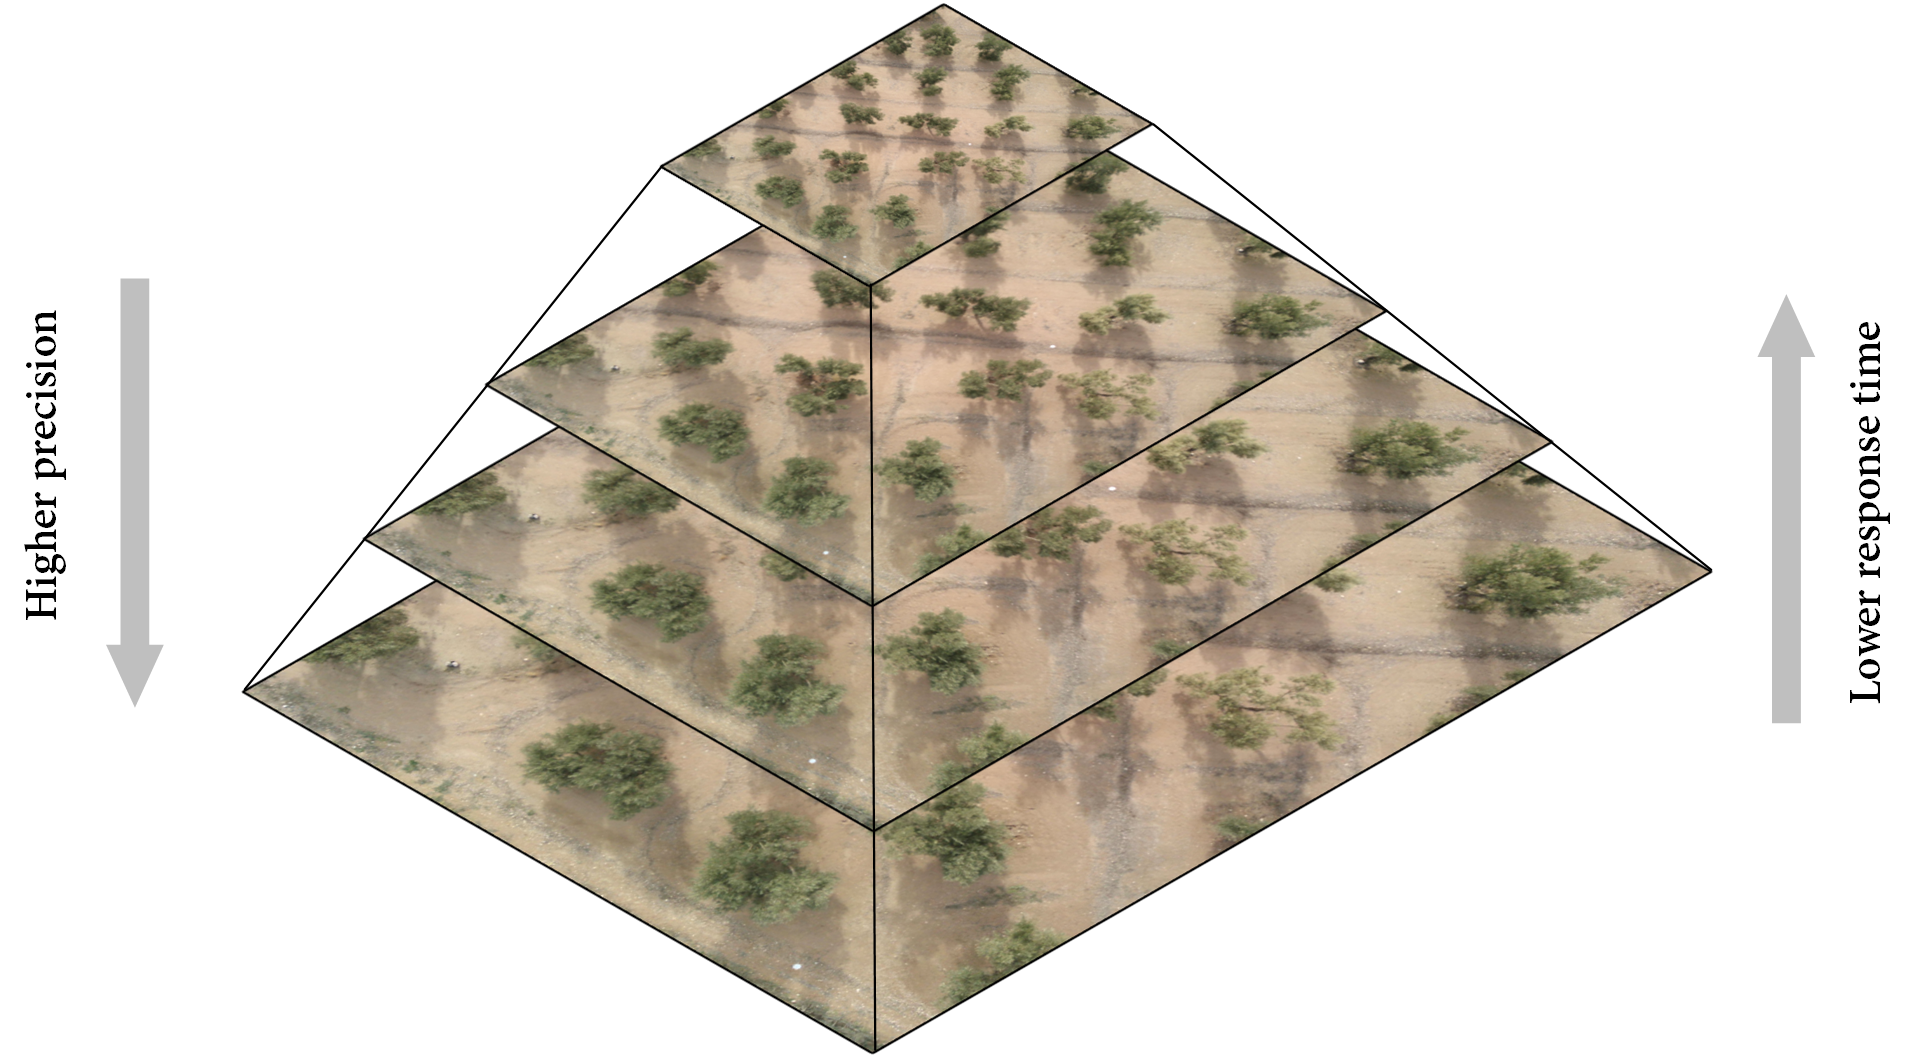
\includegraphics[width=\linewidth]{figs/conclusions/image_pyramid.png}
        \caption{Overview of an iterative image-matching algorithm, with higher image dimensionality providing slower but more fine-grained transformations.}
        \label{fig:image_pyramid}
    \end{figure}
    \item Image-matching was included as part of the reading phase in the comparisons established with commercial photogrammetry software. Therefore, this stage can be further accelerated by transferring the \acrshort{ecc} algorithm, currently obtained from OpenCV, to the \acrshort{gpu}.
    \item The generation of dense and large visible, thermal and multispectral point clouds helps to better visualize the scenario; however, point clouds with such a dimensionality are also harder to render in real-time. Although the compute-shader rendering alleviated this drawback \cite{schutz_rendering_2021}, it could be further enhanced with different levels of detail (\acrshort{lod}) \cite{schutz_gpu-accelerated_2023}. Similarly, it could help in the rendering of compressed hypercubes, since we already had to expand its real-time rendering over a few frames until completion.
    \item The compression of hypercubes was achieved by lowering the radiometric resolution with a stack-based representation, whereas spatial compression was not possible since surrounding stacks were very different. Rather than a stack-based representation, compression could be achieved in the spatial dimension, which is known to be way larger than the spectral one. 
    \item \acrshort{lidar} optimization was studied as the simplest case study: a set of optimal locations that help to survey a scene with \acrshort{tls}. However, there are other kinds of \acrshort{lidar} which may be worth exploring, such as those that rely on a path rather than a set of locations. Swarm-based optimizations may fit better if a path is required \cite{roberge_fast_2018}. Optimization of airborne \acrshort{lidar} could also be explored to determine which is the optimal configuration to densely scan a scene from a \acrshort{dsm}, including, but not limited to the followed path.
    \item A similar approach to the latter proposal is to assess \acrshort{uas} missions by computing a path that guarantees the required overlap or coverage according to the time, altitude and \acrshort{uas} flight speed, among other factors. This has been achieved for generic \acrshort{uas} missions \cite{pessacg_simplifying_2022}, though it could be further improved based on the scene geometry, represented by rapidly sketched models. It could be especially relevant for oblique view directions, by setting it as an optimizable parameter rather than a user-defined factor. 
    \item So far, the \acrshort{lidar} simulations have helped to generate large \acrshort{lidar} datasets. However, there still remain some experiments that ought to be carried out to check whether these datasets are helpful for Deep Learning tasks. Note that some of the simulated errors will be filtered out once the point clouds are voxelized, which is the most widespread approach for feeding \acrshort{lidar} datasets \cite{hackel_semantic3d_2017, behley_towards_2021}. However, it should be discerned if these synthetic datasets are similar enough to the point distribution generated by real sensors. 
    \item Part IV only explained the simulation of \acrshort{lidar} sensors, which were unavailable at that time. However, other sensors can be simulated by means of synthetically generated imagery. Generative Adversarial Networks (\acrshort{gan}) have been gaining interest as they allow building computer-made unsupervised datasets, from art to simple texts. Besides \acrshort{lidar}, infrared data could be simulated from visible imagery to create larger datasets. The current state-of-the-art has not successfully achieved this task by learning solely from visible data \cite{li_multi-branch_2019, li_i-gans_2021, kniaz_thermalgan_2019, ozkanoglu_infragan_2022, yi_cycle_2023}, since it may require semantic annotations to isolate surfaces that have different radiance. 
    \begin{figure}
    \centering
    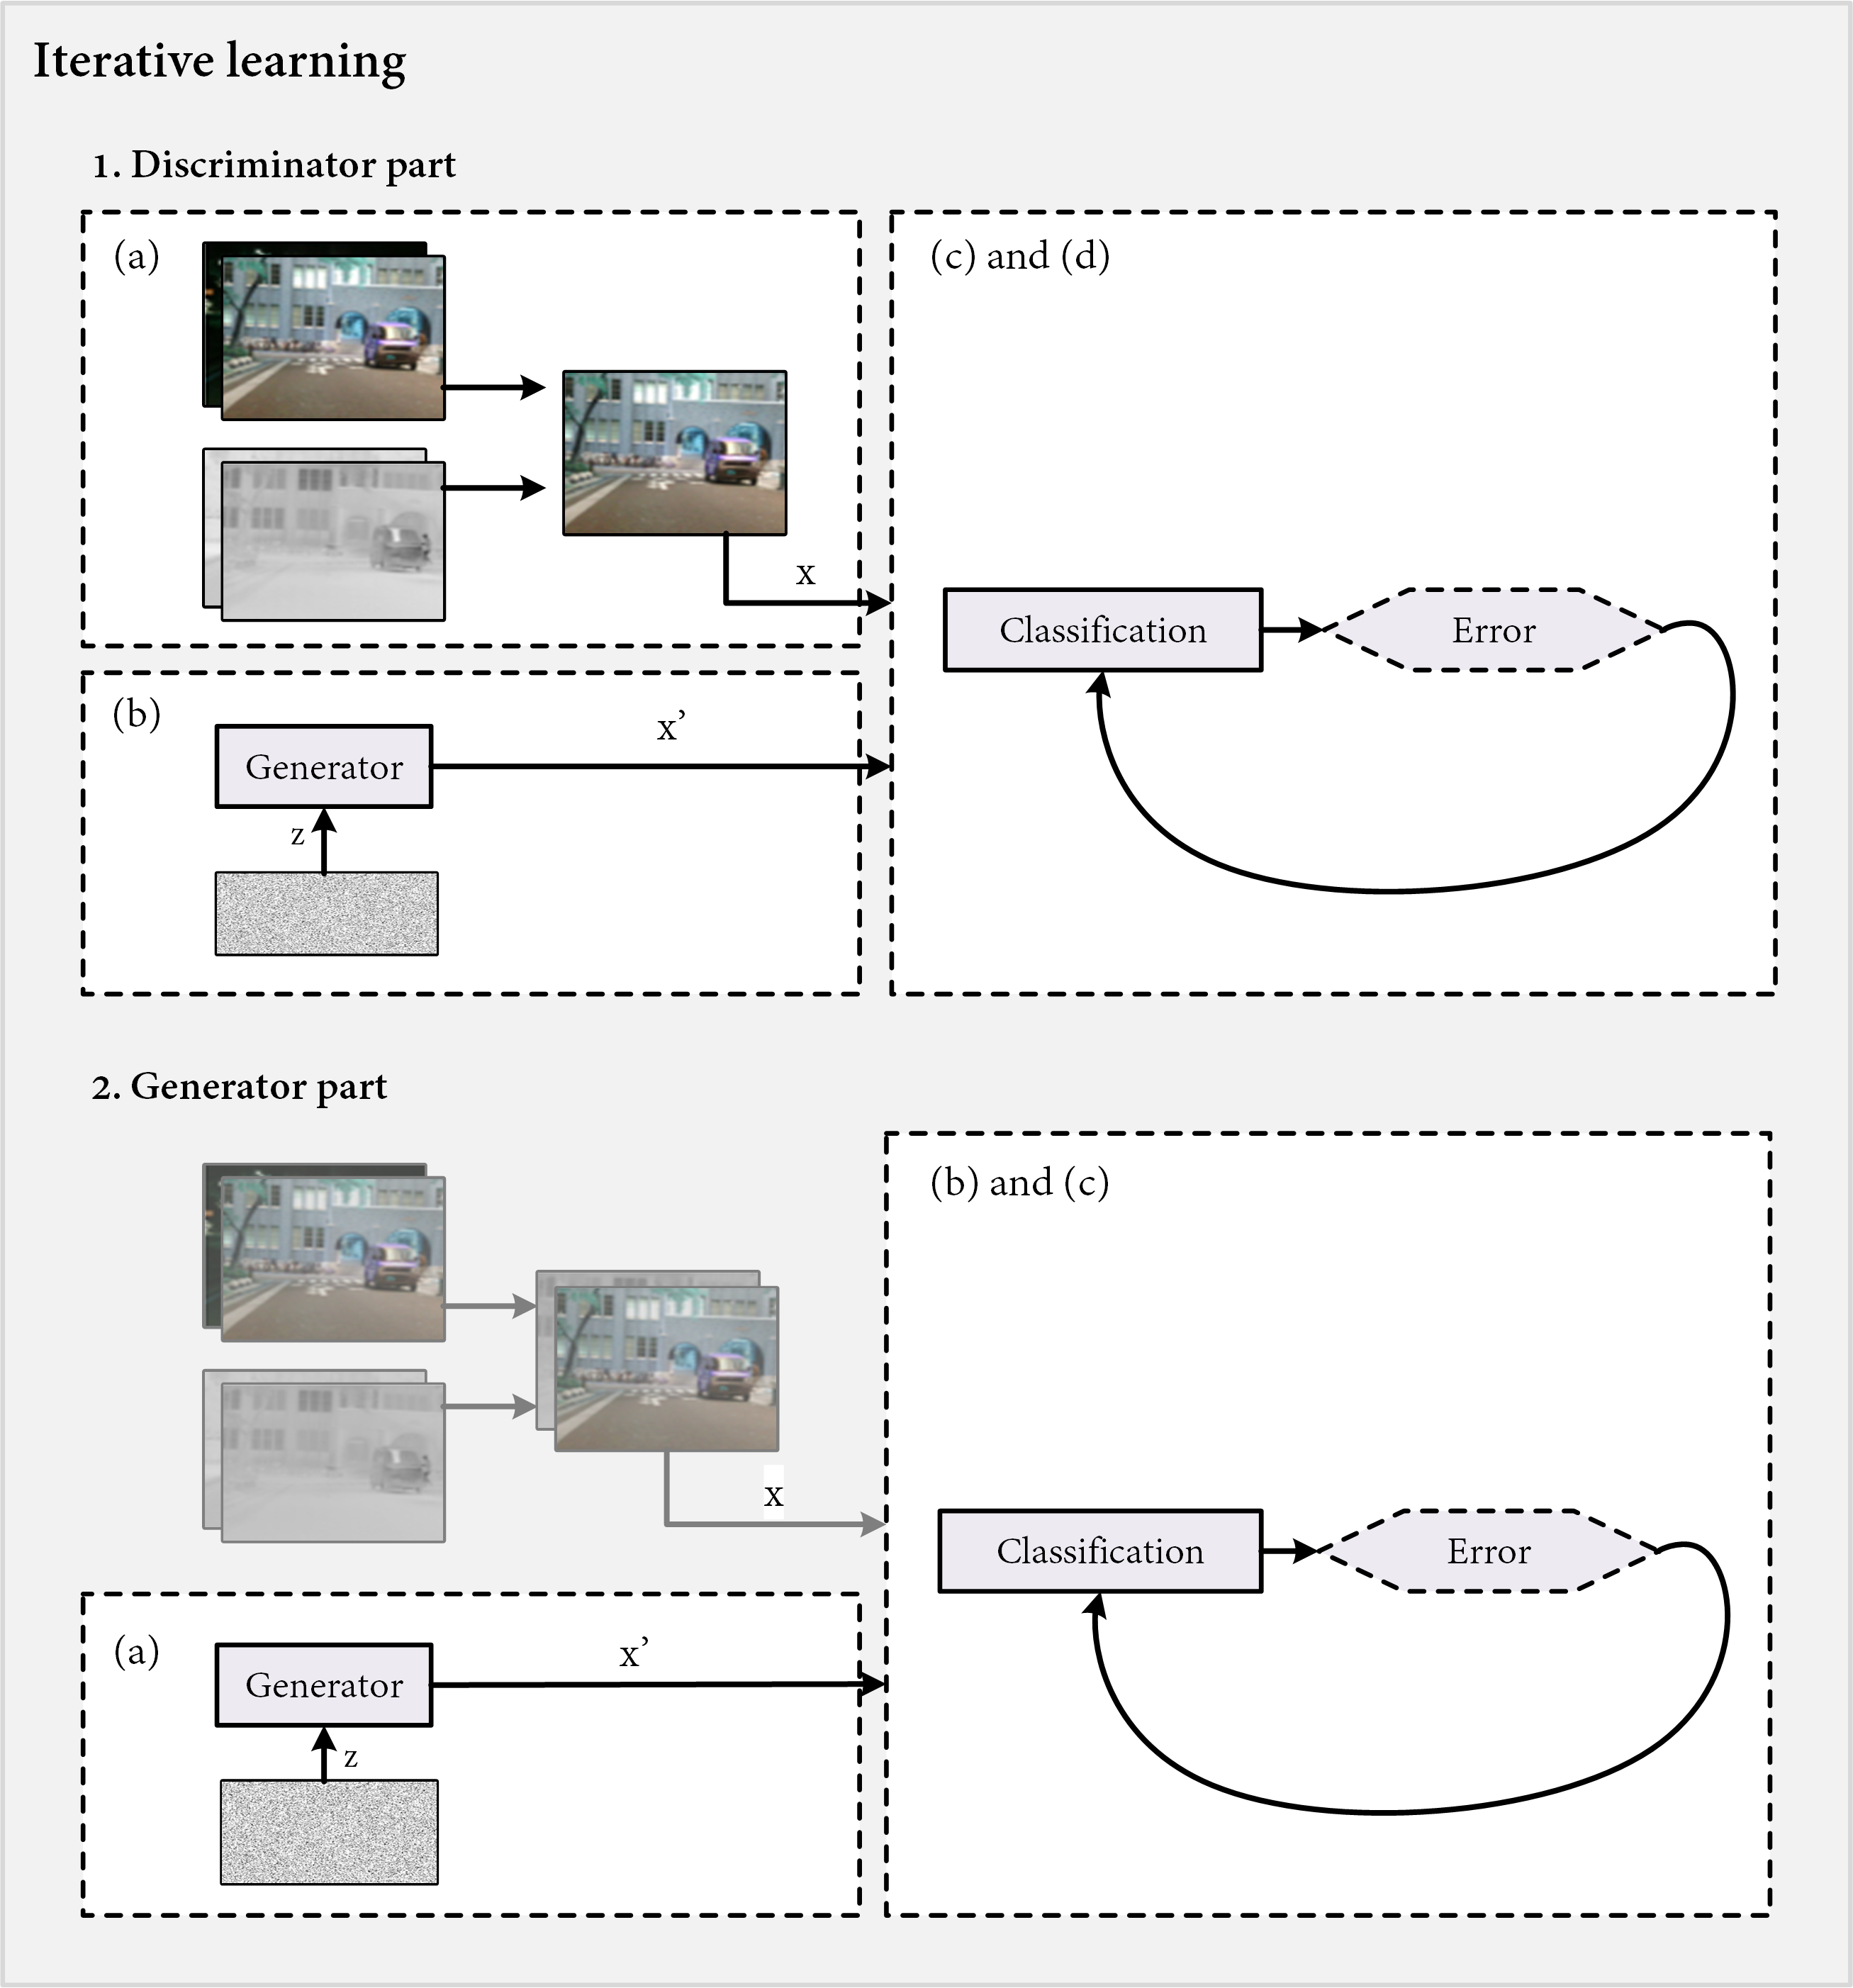
\includegraphics[width=\linewidth]{figs/conclusions/gan.png}
    \caption{Overview of the proposed \acrshort{lidar} simulation. First, scenes are modelled either as static or procedural, linked to semantic labels as well as to materials properties. Then, a virtual \acrshort{lidar} iteratively solves the simulation and its result is stored in a standard file format.}
    \label{fig:conclusions_gan}
\end{figure}
    \item The phenotyping of grapevine varieties was approached with Deep Learning; however, this model could be improved by further integrating more varieties and collecting datasets at different stages of the year. Also, there are other interesting approaches to address this very same task, from multi-instance \cite{meerdink_multitarget_2022} to contrastive learning \cite{guan_spatial-spectral_2022}. 
\end{itemize}